%%%%%%%%%%%%%%%%%%%%%%%%%%%%%%%%%%%%%%%%%
% Classicthesis-Styled CV
% LaTeX Template
% Version 1.0 (22/2/13)
%
% This template has been downloaded from:
% http://www.LaTeXTemplates.com
%
% Original author:
% Alessandro Plasmati
%
% License:
% CC BY-NC-SA 3.0 (http://creativecommons.org/licenses/by-nc-sa/3.0/)
%
%%%%%%%%%%%%%%%%%%%%%%%%%%%%%%%%%%%%%%%%%

%----------------------------------------------------------------------------------------
%	PACKAGES AND OTHER DOCUMENT CONFIGURATIONS
%----------------------------------------------------------------------------------------

\documentclass[xcolor=dvipsnames]{scrartcl}

\usepackage{graphicx}

\usepackage[dvipsnames]{xcolor}
\definecolor{myblue}{RGB}{0,128,255}
\reversemarginpar % Move the margin to the left of the page 
%\textwidth = 597pt%\usepackage[margin=0.5in]{geometry}

\usepackage[T1]{fontenc}
\usepackage[utf8]{inputenc}
\usepackage{textcomp}

%\renewcommand{\rmdefault}{phv}

\newcommand{\MarginText}[1]{\marginpar{\raggedleft\itshape\small#1}} % New command defining the margin text style

\usepackage[nochapters]{classicthesis} % Use the classicthesis style for the style of the document
\usepackage[LabelsAligned]{currvita} % Use the currvita style for the layout of the document
\usepackage{fontawesome}


\renewcommand{\cvheadingfont}{\Huge\color{myblue}} % Font color of your name at the top

\usepackage{hyperref} % Required for adding links	and customizing them
%\hypersetup{colorlinks, breaklinks, urlcolor=RoyalBlue, linkcolor=RoyalBlue} % Set link colors

\newlength{\datebox}\settowidth{\datebox}{MonthYearXXXXX} % Set the width of the date box in each block

\newlength{\iconbox}\settowidth{\iconbox}{GIFT} % Set the width of the date box in each block

\newcommand{\NewEntry}[3]{\noindent\hangindent=2em\hangafter=0  \parbox{\datebox}{\textit{#1}}\hspace{0.5em} #2 #3 % Define a command for each new block - change spacing and font sizes here: #1 is the left margin, #2 is the italic date field and #3 is the position/employer/location field
\vspace{0.5em}} % Add some white space after each new entry

\newcommand{\NewInfo}[2]{\noindent\hangindent=2em\hangafter=0  \parbox{\iconbox}#1\hspace{0.5em} #2 % Define a command for each new block - change spacing and font sizes here: #1 is the left margin, #2 is the italic date field and #3 is the position/employer/location field
\vspace{0.5em}} % Add some white space after each new entry

\newcommand{\Description}[1]{\hangindent=2em\hangafter=0\noindent\raggedright\footnotesize{#1}\par\normalsize\vspace{1em}} % Define a command for descriptions of each entry - change spacing and font sizes here
\usepackage{vmargin}
\setmarginsrb           { 2cm}  % left margin
                        { 0.6in}  % top margin
                        { 2cm}  % right margin
                        { 0.8in}  % bottom margin
                        { 12pt}  % head height
                        { 9pt}  % head sep
                        {   9pt}  % foot height
                        { 0.3in}  % foot sep

%----------------------------------------------------------------------------------------

\begin{document}

\thispagestyle{empty} % Stop the page count at the bottom of the first page

%----------------------------------------------------------------------------------------
%	NAME AND CONTACT INFORMATION SECTION
%----------------------------------------------------------------------------------------



%\hfill

%\begin{minipage}{0.6\textwidth}\raggedleft

\begin{cv}{\spacedallcaps{David Handl}}\vspace{1.5em} % Your name

\begin{minipage}{0.7\textwidth}%\centering
\noindent\spacedlowsmallcaps{Experimental Particle Physicist}\vspace{0.5em}% Personal information heading

\NewInfo{\faGift}{Born in Austria, 26$^{\mathrm{th}}$ May, 1989}% Birthplace and date

\NewInfo{\faHome}{Breisacher Stra{\ss}e 30, 81667 Munich, Germany}

%\NewEntry{\faEnvelope}{\href{mailto:david.handl@cern.ch}{david.handl@cern.ch}} % Email address
\NewInfo{\faEnvelope}{\href{mailto:handl.david89@gmail.com}{handl.david89@gmail.com}} % Email address

%\NewEntry{website}{\href{http://www.hephy.at/en/hephy/staff-members/detail/name/handl/}{http://www.hephy.at/en/hephy/staff-members/detail/name/handl/}} % Personal website

\NewInfo{\faPhone}{+49 177 411 300 9 }%\ \ $\cdotp$\ \ (M) +1 (000) 111 1112} % Phone number(s)

\NewInfo{\faGithub}{\href{https://github.com/dhandl}{https://github.com/dhandl}} % Email address

\end{minipage}
\begin{minipage}{0.25\textwidth}%\raggedleft% adapt widths of minipages to your needs
  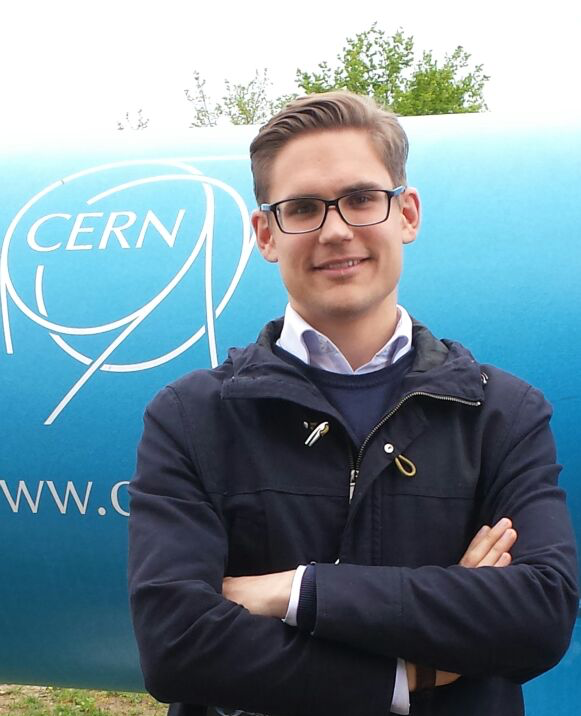
\includegraphics[width=0.9\textwidth]{dhandl.png}
\end{minipage}


\vspace{1em} % Extra white space between the personal information section and goal

\noindent\spacedlowsmallcaps{\color{myblue}Core competencies}\vspace{0.5em} % Goal heading, could be used for a quotation or short profile instead

\Description{Excellent analytical skills of large-scale data\ \ $\cdotp$\ \ In-depth knowledge of advanced statistics and mathematics\ \ $\cdotp$\ \ Vital skills in computer science as well as strong expertise in programming languages such as C, C++ and Python, etc.\ \ $\cdotp$\ \ Excellent experience in the fundamentals of machine learning and libraries such as Keras and tensorflow, etc.\ \ $\cdotp$\ \ Substantial know-how to work collaboratively as a member of an international team\ \ $\cdotp$\ \ Very good education in fundamental physics and in-depth knowledge in particle physics\ \ $\cdotp$\ \ Proven leadership abilities during the technical supervision of undergraduate students\ \ $\cdotp$\ \ Strongly motivated, communicative and cooperative appearance}\vspace{1em} % competencies text

%----------------------------------------------------------------------------------------
%	WORK EXPERIENCE
%----------------------------------------------------------------------------------------

\noindent\spacedlowsmallcaps{\color{myblue}\textsf{Research}}\vspace{0.5em}

\NewEntry{May~'16-Present}{Ph.D. Student, Faculty of Physics, Ludwig-Maximilians-Universit\"at M\"unchen -- Munich}

\Description{As an ambitous member of the ATLAS Collaboration, I am actively contributing to the statistical data analysis of a search for supersymmetry in single lepton final states. I am studying the capability of novel deep learning algorithms to enhance the search sensitivity. In order to separate signal from background events, I developed a powerful classifier based on recurrent as well as deep neural networks. Apart from that, I investigated potential improvements of the missing transverse energy high level object trigger system. In addition, I spent six months of my research abroad at the European Organization for Nuclear Research (CERN) in Geneva, Switzerland, to get a detailed insight of internal operations and the work life at an international research environment. Since I am strongly dedicated in outreach affairs, I also took the chance to become an official visitor guide for several experiments and facilities, including the ATLAS underground cavern. During the technical supervision of serveral undergraduate students, I strengthened my leadership abilities. I am also a tutor for particle physics exercise courses at the LMU Munich and I am volunteering as a tutor at physics masterclasses.\\}

\NewEntry{Oct~'14-Dec~'15}{Master Student, Institute of High Energy Physics -- Vienna}

\Description{As a master student I worked as an active member in a joint collaboration consisting of data analysis groups at the University of Athens, CERN, DESY Hamburg and the Institute of High Energy Physics in Vienna. We performed searches for supersymmetry in single lepton final states using $13$ TeV data recorded by the CMS collaboration. I made significant contributions to the estimation of the dominant standard model backgrounds.}% in final states with $0$ b-tagged jets, I investigated several kinematic variables to supress the main backgrounds and I also performed studies on systematic uncertainties.}% Reference: John \textsc{McDonald}\ \ $\cdotp$\ \ +1 (000) 111 1111\ \ $\cdotp$\ \ \href{mailto:john@lehman.com}{john@lehman.com}}

%------------------------------------------------

\NewEntry{Sept-Oct 2014}{Intern, Institute of High Energy Physics  -- Vienna}

\Description{As an intern in the hardware group, I performed electrical tests of the readout electronics for the Belle II Silicon Vertex Detector. Several important quality coefficients of the readout chips were measured and a statistical evaluation was performed. Based on these tests faulty readout chips could be localised and were sorted out.\\}% Reference: Bill \textsc{Lumbergh}\ \ +1 (000) 111 1111\ \ $\cdotp$\ \ \href{mailto:bill@initech.com}{bill@initech.com}}

%------------------------------------------------

\NewEntry{Oct-Dec 2013}{Intern, Institute of High Energy Physics -- Vienna}

\Description{During my first internship at the Institute of High Energy Physics, I got involved in the data analysis group where I improved a search for supersymmetry using neural networks. Thus, I performed the parameter optimisation of neural networks and studied various performance measures in order to get a deeper understanding of the model evaluation.}%Results showed that including event shape variables to a certain collection of kinematic variables led to a slight improvement of signal efficiency.\\}% Reference: Big \textsc{Mike}\ \ +1 (000) 111 1111\ \ $\cdotp$\ \ \href{mailto:mike@buymore.com}{mike@buymore.com}}

%------------------------------------------------

\vspace{1em} % Extra space between major sections
%\newpage
%\thispagestyle{empty}
%----------------------------------------------------------------------------------------
%	PUBLICATIONS
%----------------------------------------------------------------------------------------

\noindent\spacedlowsmallcaps{\color{myblue}Publications}\vspace{0.5em}

%\NewEntry{2017}{~}

\Description{\textit{Search for direct top squark pair production in the 3-body decay mode with a final state containing one lepton, jets, and missing transverse momentum in $\sqrt{s}=13$~TeV $pp$ collision data with the ATLAS detector}, ATLAS Conference Note (\texttt{https://cds.cern.ch/record/2676594})\\} 

\Description{\textit{Search for top squark pair production in final states with one isolated lepton, jets, and missing transverse momentum using 36~$fb^{-1}$ of $\sqrt{s}=13$~TeV $pp$ collision data with the ATLAS detector}, in Journal of High Energy Physics (\texttt{DOI:10.1007/JHEP06(2018)108})\\}

\Description{\textit{Search for top squarks in final states with one electron or muon in $\sqrt{s}=13$~TeV $pp$ collisions with the ATLAS detector}, in Proceedings of Science 2017 (\texttt{https://pos.sissa.it/314/699/pdf})\\}

\vspace{1em} % Extra space between major sections

%----------------------------------------------------------------------------------------
%	Talks and posters
%----------------------------------------------------------------------------------------

\noindent\spacedlowsmallcaps{\color{myblue}Talks and posters}\vspace{0.5em}

%\NewEntry{2018}{~}

\Description{\textit{Applications of Machine Learning techniques at the ATLAS collaboration}, string\_data18 Workshop, March 2018\\}

%\NewEntry{2017}{~}

\Description{\textit{Search for top squarks in final states with one electron or muon in $\sqrt{s}=13$~TeV $pp$ collisions with the ATLAS detector}, EPS-HEP, July 2017\\}

\vspace{1em} % Extra space between major sections


%----------------------------------------------------------------------------------------
%	EDUCATION
%----------------------------------------------------------------------------------------

\noindent\spacedlowsmallcaps{\color{myblue}Education}\vspace{0.5em}

\NewEntry{August 2018}{\textsc{Hadron Collider Physics Summer School at Fermilab}}

\Description{I entered one of the most prestigious summer schools about high energy physics at Fermilab, Batavia, Illinois.}

\NewEntry{2016-Present}{\textsc{Ludwig-Maximilians-Universit\"at M\"unchen}}

\Description{Ph.D. candidate in Physics}
%Thesis: (tentative title)\textit{Search for stop quark pair production in the single lepton final state in 13 TeV pp collisions with the ATLAS detector}\newline
%Supervisor: \textit{Prof.~Dorothee Schaile \& Dr.~Jeannine Wagner-Kuhr}\newline}

\NewEntry{2013-2016}{\textsc{Vienna University of Technology}}

\Description{M.Sc. in Technical Physics}
%Thesis: \textit{Background estimation for searches for supersymmetry in the single lepton final state in 13 TeV pp collisions}\newline
%Supervisor: \textit{Prof.~Jochen Schieck \& Dr.~Robert Sch\"ofbeck}\newline}
%Description: My thesis presents a search for supersymmetry with exactly one lepton, multiple jets and no b tagged jet in the final state with $13\rm{TeV}$ data taken in $2015$. The angle between the lepton and the W boson direction is used as the main discriminative variable. The central element of the thesis is the estimation of the most important backgrounds from control regions in data. The search is performed in exclusive regions based on the sum of the transverse momenta of all jets as well as the sum of the missing transverse energy and the lepton momentum.\newline}
%Advisors: Prof.~Jochen Schieck \& Dr.~Wolfgang Adam}

%------------------------------------------------

\NewEntry{2009-2013}{\textsc{Vienna University of Technology}}

\Description{B.Sc. in Technical Physics}
%Thesis: \textit{Implementation and optimization of an electrospray deposition system}\newline
%Supervisor: \textit{Prof. Ulrike Diebold}\newline}
%Description: I designed and implemented a purge chamber to optimize an electrospray depostion system. The electrospray was used to adsorb molecules on oxide surfaces. Tests showed that the implementation led to a significant increase of the purity of the molecular beam.\newline}
%Advisors: Prof.~Ulrike Diebold}
%------------------------------------------------

\vspace{1em} % Extra space between major sections

%----------------------------------------------------------------------------------------
%	PUBLICATIONS
%----------------------------------------------------------------------------------------

%\spacedlowsmallcaps{Publications}\vspace{1em}

%\NewEntry{June 2015}{Search for Supersymmetry in events with one lepton}

%\Description{\MarginText{CMS-AN-14-288 internal analysis note}We present a strategy for an early inclusive single lepton search with 13 TeV data. We require a high threshold for the sum of missing transverse momentum and the transverse momentum of the lepton, which makes the search sensitive to R-parity conserving supersymmetry. We further use the search variable $\Delta\Phi$ to suppress the background. To optimize the sensitivity to various new physics topologies, we search in several exclusive categories, which differ in the number of jets and btags. To be less dependent on the new physiscs scale we also introduce separate search categories based on the sum of all jet transverse momenta and on the sum of the transverse missing momentum and the lepton.}%\\ Authors: John \textsc{Smith}, ~James \textsc{Smith}}

%------------------------------------------------

%\NewEntry{October 2015}{Search for Supersymmetry with single-lepton events at 13 TeV using 2015 data}

%\Description{\MarginText{CMS-AN-15-207 internal analysis note}We present an inclusive single-lepton search with 13 TeV data taken in 2015. To optimize the sensitivity to various new physics topologies, we search in several exclusive categories, which differ in the number of jets and b-tagged jets.  We further use the angle between the lepton and the W boson direction, $\Delta\Phi$, to suppress the background. To be less dependent on the new physics scale we also introduce separate search categories based on the sum of all jet transverse momenta and on the sum of the transverse missing momentum and the lepton.}%\\ Authors: John \textsc{Smith}, ~James %\textsc{Smith}}

%------------------------------------------------

%\vspace{1em} % Extra space between major sections

%----------------------------------------------------------------------------------------
%	COMPUTER SKILLS
%----------------------------------------------------------------------------------------

\noindent\spacedlowsmallcaps{\color{myblue}Computing Skills}\vspace{0.5em}

%\Description{\MarginText{Intermediate}\textsc{C++}}
\Description{C, C++, Python, keras, tensorflow, scikit-learn, MATLAB, ROOT, Linux, Github, Latex, MS Office}
%\Description{\MarginText{Advanced}\textsc{python}, \LaTeX, Linux}

%\Description{\MarginText{Advanced}Computer Hardware and Support}

%------------------------------------------------

\vspace{1em} % Extra space between major sections

%----------------------------------------------------------------------------------------
%	OTHER INFORMATION
%----------------------------------------------------------------------------------------

\noindent\spacedlowsmallcaps{\color{myblue}Other Information}\vspace{0.5em}

%\Description{\MarginText{Awards}2011\ \ $\cdotp$\ \ School of Business Postgraduate Scholarship}

%\vspace{-0.5em} % Negative vertical space to counteract the vertical space between every \Description command

%\Description{2010\ \ $\cdotp$\ \ Top Achiever Award -- Commerce}

%------------------------------------------------

%\vspace{1em}

%\Description{\MarginText{Communication Skills}2010\ \ $\cdotp$\ \ Oral Presentation at the California Business Conference}

%\vspace{-0.5em} % Negative vertical space to counteract the vertical space between every \Description command

%\Description{2009\ \ $\cdotp$\ \ Poster at the Annual Business Conference in Oregon}

%------------------------------------------------

\vspace{1em}

\newlength{\langbox} % Create a new length for the length of languages to keep them equally spaced
\settowidth{\langbox}{English} % Length equals the length of "English" - if you have a longer language in your list put it here

\NewEntry{Languages}{~}

\Description{\parbox{\langbox}{\textsc{German}}\ \ $\cdotp$\ \ \ Mothertongue}

\vspace{-0.5em} % Negative vertical space to counteract the vertical space between every \Description command

\Description{\parbox{\langbox}{\textsc{English}}\ \ $\cdotp$\ \ \ Advanced }%(conversationally fluent)}

\vspace{-0.5em} % Negative vertical space to counteract the vertical space between every \Description command

\Description{\parbox{\langbox}{\textsc{French}}\ \ $\cdotp$\ \ \ Basic (simple words and phrases only)}

\vspace{0.5em} % Negative vertical space to counteract the vertical space between every \Description command

%------------------------------------------------

\NewEntry{Interests}{~}

\Description{running\ \ $\cdotp$\ \ skiing\ \ $\cdotp$\ \ football\ \ $\cdotp$\ \ reading\ \ $\cdotp$\ \ cooking\ \ $\cdotp$\ \ programming\ \ $\cdotp$\ \ photography}

%----------------------------------------------------------------------------------------

\end{cv}

\end{document}
